\chapter{Implementacija i korisničko sučelje}
		
		
		\section{Korištene tehnologije i alati}
		
			Tim je koristio \underline{WhatsApp}.\footnote[1]{https://www.whatsapp.com/} i \underline{Notion}.\footnote[2]{https://www.notion.so/} za komunikaciju unutar tima. Za izradu UML dijagrama korišten je \underline{Astah Professional}.\footnote[3]{https://astah.net/products/astah-professional/}, dok je za upravljanje izvornim kodom odabran \underline{Git}.\footnote[4]{https://git-scm.com/}. Udaljeni repozitorij projekta dostupan je na web platformi \underline{GitHub}.\footnote[5]{https://github.com/}.
			
			Kao razvojna okruženja korišteni su \underline{Visual Studio Code}.\footnote[6]{https://code.visualstudio.com/} i \underline{IntelliJ IDEA}.\footnote[7]{https://www.jetbrains.com/idea/}. Visual Studio Code je jednostavan uređivač koda s podrškom za razvojne operacije poput debugiranja, pokretanja zadataka i kontrolu verzija od tvrtke Microsoft, dok je IntelliJ popularno razvojno okruženje (IDE) razvijeno od strane tvrtke JetBrains. Namijenjeno je prvenstveno za rad s Java programskim jezikom.
			
			Aplikacija je napisana koristeći radni okvir \underline{Spring Boot}.\footnote[8]{https://spring.io/projects/spring-boot/} i jezik \underline{Java}.\footnote[9]{https://www.java.com/en/} za izradu backenda te \underline{React}.\footnote[10]{https://react.dev/} i jezik \underline{JavaScript}.\footnote[11]{https://www.javascript.com/} za izradu frontenda. React je besplatna i open-source JavaScript biblioteka za izgradnju korisničkih sučelja temeljenih na komponentama. Održava je Meta i zajednica pojedinačnih razvijatelja te tvrtki. Radni okvir Spring Boot je otvoreni, mikroservisni Java web okvir koji nudi Spring. Razvijen je kako bi pojednostavio proces izrade, konfiguracije i razmještanja Java aplikacija. 
			
			Baza podataka se nalazi na posluzitelju u oblaku \underline{Render}.\footnote[12]{https://render.com/}.
			
			
			\eject 
		
	
		\section{Ispitivanje programskog rješenja}
			\section{Ispitivanje komponenti}
			
			Sveobuhvatan pregled našeg testiranja temeljio se na korištenju JUnit 5 za izvođenje unit testova. Većina testova odnosi se na ispitivanje ispravnosti podataka u Dto objektima (ActionDto, AnimalDto, AvailableSearcherDto, RequestDto i TaskDto). Jedan od ispitivanja služi za provjeru ispravnog formata maila, a jedan za provjeru ispravnosti koordinata. Zadnje od ispitivanja provjerava ispravnost funkcije koja služi za micanje tragača s akcije.
			
			\subsection{Ispitivanje funkcije checkActionDto:}
			Provjerava se funkcionalnost metode \textit{checkActionDto} u \textit{researcherServiceJpa servisu} koja služi za provjeru ispravnosti podataka unutar \textit{ActionDto} objekta.
			
			\textbf{testCheckActionDtoValid:}
			\begin{itemize}
				\item U funkciju se šalje objekt \textit{ActionDto} s ispravnim podacima.
				\item Očekuje se da neće doći do bacanja iznimke.
			\end{itemize}
			\begin{lstlisting}
				@Test
				public void testCheckActionDtoValid() {
					ActionDto validActionDto = new ActionDto(1L, "ActionName", "ActionType", "LocationName");
					assertDoesNotThrow(() -> researcherServiceJpa.checkActionDto(validActionDto));
				}
			\end{lstlisting}
			
			\textbf{testCheckActionDtoInvalidNull:}
			\begin{itemize}
				\item U funkciju se šalje objekt \textit{ActionDto} s neispravnim podacima (\textit{actionName} postavljen na \textit{null}).
				\item Očekuje se da će doći do bacanja iznimke.
			\end{itemize}
			\begin{lstlisting}
				@Test
				public void testCheckActionDtoInvalidNull() {
					ActionDto invalidActionDto = new ActionDto(null, null, "ActionType", "LocationName");
					assertThrows(IllegalArgumentException.class, () -> researcherServiceJpa.checkActionDto(invalidActionDto));
				}
			\end{lstlisting}
			
			\textbf{testCheckActionDtoInvalidEmpty:}
			\begin{itemize}
				\item U funkciju se šalje objekt \textit{ActionDto} s neispravnim podacima (\textit{actionName} postavljen na \textit{""}).
				\item Očekuje se da će doći do bacanja iznimke.
			\end{itemize}
			\begin{lstlisting}
				@Test
				public void testCheckActionDtoInvalidEmpty() {
					ActionDto invalidActionDto = new ActionDto(1L, "", "ActionType", "LocationName");
					assertThrows(IllegalArgumentException.class, () -> researcherServiceJpa.checkActionDto(invalidActionDto));
				}
			\end{lstlisting}
			
			\textbf{testCheckActionDtoInvalidWhitespace:}
			\begin{itemize}
				\item U funkciju se šalje objekt \textit{ActionDto} s neispravnim podacima (\textit{actionName} postavljen na \textit{" ActionName"}).
				\item Očekuje se da će doći do bacanja iznimke.
			\end{itemize}
			\begin{lstlisting}
				@Test
				public void testCheckActionDtoInvalidWhitespace() {
					ActionDto invalidActionDto = new ActionDto(1L, " ActionName", "ActionType", "LocationName");
					assertThrows(IllegalArgumentException.class, () -> researcherServiceJpa.checkActionDto(invalidActionDto));
				}
			\end{lstlisting}
			
			\begin{figure}[H]
				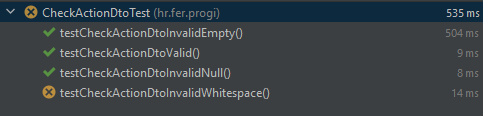
\includegraphics[scale=1]{slike/checkActionDtoTest.png} 
				\centering
				\caption{Rezultati ispitivanja}
				\label{fig:promjene}
			\end{figure}
			
			\subsection{Ispitivanje funkcije checkAnimalDto:}
			Provjerava se funkcionalnost funkcije \textit{checkAnimalDto} u \textit{SearcherInTheFieldJpa servisu} koja služi za provjeru ispravnosti podataka unutar \textit{AnimalDto} objekta.
			
			\textbf{testCheckAnimalDtoValid:}
			\begin{itemize}
				\item U funkciju se šalje objekt \textit{AnimalDto} s ispravnim podacima.
				\item Očekuje se da neće doći do bacanja iznimke.
			\end{itemize}
			\begin{lstlisting}
				@Test
				public void testCheckAnimalDtoValid() {
					
					AnimalDto validAnimalDto = new AnimalDto();
					validAnimalDto.setAnimalName("Vuk");
					validAnimalDto.setBreed("Licki");
					validAnimalDto.setDescription("Sivi, brzi vuk");
					validAnimalDto.setCurrentPosition(Arrays.asList(1.0, 2.0));
					
					assertDoesNotThrow(() -> searcherJpa.checkAnimalDto(validAnimalDto));
				}
			\end{lstlisting}
			
			\textbf{testCheckAnimalDtoNull:}
			\begin{itemize}
				\item U funkciju se šalje objekt \textit{AnimalDto} postavljen na \textit{null}.
				\item Očekuje se da će doći do bacanja iznimke.
			\end{itemize}
			\begin{lstlisting}
				@Test
				public void testCheckAnimalDtoNull() {
					AnimalDto nullAnimalDto = null;
					
					IllegalArgumentException exception = assertThrows(IllegalArgumentException.class,
					() -> searcherJpa.checkAnimalDto(nullAnimalDto));
					
					assertEquals("AnimalDto is null", exception.getMessage());
				}
			\end{lstlisting}
			
			\textbf{testCheckAnimalDtoMissingName:}
			\begin{itemize}
				\item U funkciju se šalje objekt \textit{AnimalDto} s neispravnim podacima (nedostaje varijabla \textit{AnimalName}).
				\item Očekuje se da će doći do bacanja iznimke.
			\end{itemize}
			\begin{lstlisting}
				@Test
				public void testCheckAnimalDtoMissingName() {
					AnimalDto missingNameDto = new AnimalDto();
					missingNameDto.setBreed("Licki");
					missingNameDto.setDescription("Sivi, brzi vuk");
					missingNameDto.setCurrentPosition(Arrays.asList(1.0, 2.0));
					
					IllegalArgumentException exception = assertThrows(IllegalArgumentException.class,
					() -> searcherJpa.checkAnimalDto(missingNameDto));
					
					assertEquals("AnimalName is missing", exception.getMessage());
				}
			\end{lstlisting}
			
			\textbf{testCheckAnimalDtoMissingBreed:}
			\begin{itemize}
				\item U funkciju se šalje objekt \textit{AnimalDto} s neispravnim podacima (nedostaje varijabla \textit{Breed}).
				\item Očekuje se da će doći do bacanja iznimke.
			\end{itemize}
			\begin{lstlisting}
				@Test
				public void testCheckAnimalDtoMissingBreed() {
					AnimalDto missingBreedDto = new AnimalDto();
					missingBreedDto.setAnimalName("Vuk");
					missingBreedDto.setDescription("Sivi, brzi vuk");
					missingBreedDto.setCurrentPosition(Arrays.asList(1.0, 2.0));
					
					IllegalArgumentException exception = assertThrows(IllegalArgumentException.class,
					() -> searcherJpa.checkAnimalDto(missingBreedDto));
					
					assertEquals("Breed is missing", exception.getMessage());
				}
			\end{lstlisting}
			
			\begin{figure}[H]
				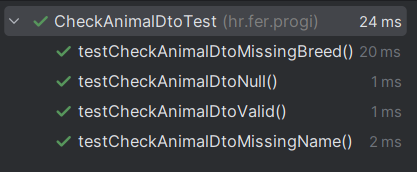
\includegraphics[scale=1]{slike/checkAnimalDtoTest.png} 
				\centering
				\caption{Rezultati ispitivanja}
				\label{fig:checkAnimalDtoTest}
			\end{figure}
			
			\subsection{Ispitivanje funkcije checkAvailableSearcherDto:}
			Provjerava se funkcionalnost funkcije \textit{checkAvailableSearcherDto} u \textit{StationManagerJpa servisu} koja služi za provjeru ispravnosti podataka unutar \textit{AvailableSearcherDto} objekta.
			
			\textbf{testCheckAvailableSearcherDtoValid:}
			\begin{itemize}
				\item U funkciju se šalje objekt \textit{AvailableSearcherDto} s ispravnim podacima.
				\item Očekuje se da neće doći do bacanja iznimke.
			\end{itemize}
			\begin{lstlisting}
				@Test
				public void testCheckAvailableSearcherDtoValid() {
					AvailableSearcherDto validSearcherDto = new AvailableSearcherDto();
					validSearcherDto.setFirstName("John");
					validSearcherDto.setLastName("Doe");
					validSearcherDto.setQualification("Biologist");
					validSearcherDto.setCurrentPosition(Arrays.asList(1.0, 2.0));
					
					assertDoesNotThrow(() -> stationManagerJpa.checkAvailableSearcherDto(validSearcherDto));
				}
			\end{lstlisting}
			
			\textbf{testCheckAvailableSearcherDtoNull:}
			\begin{itemize}
				\item U funkciju se šalje objekt \textit{AvailableSearcherDto} postavljen na \textit{null}.
				\item Očekuje se da će doći do bacanja iznimke.
			\end{itemize}
			\begin{lstlisting}
				@Test
				public void testCheckAvailableSearcherDtoNull() {
					AvailableSearcherDto nullSearcherDto = null;
					
					IllegalArgumentException exception = assertThrows(IllegalArgumentException.class,
					() -> stationManagerJpa.checkAvailableSearcherDto(nullSearcherDto));
					
					assertEquals("AvailableSearcherDto is null", exception.getMessage());
				}
			\end{lstlisting}
			
			\textbf{testCheckAvailableSearcherDtoMissingFirstName:}
			\begin{itemize}
				\item U funkciju se šalje objekt \textit{AvailableSearcherDto} s neispravnim podacima (nedostaje varijabla \textit{FirstName}).
				\item Očekuje se da će doći do bacanja iznimke.
			\end{itemize}
			\begin{lstlisting}
				@Test
				public void testCheckAvailableSearcherDtoMissingFirstName() {
					AvailableSearcherDto missingFirstNameDto = new AvailableSearcherDto();
					missingFirstNameDto.setLastName("Doe");
					missingFirstNameDto.setQualification("Biologist");
					missingFirstNameDto.setCurrentPosition(Arrays.asList(1.0, 2.0));
					
					IllegalArgumentException exception = assertThrows(IllegalArgumentException.class,
					() -> stationManagerJpa.checkAvailableSearcherDto(missingFirstNameDto));
					
					assertEquals("First name is missing", exception.getMessage());
				}
			\end{lstlisting}
			
			\textbf{testCheckAvailableSearcherDtoMissingCurrentPosition:}
			\begin{itemize}
				\item U funkciju se šalje objekt \textit{AvailableSearcherDto} s neispravnim podacima (nedostaje varijabla \textit{CurrentPosition}).
				\item Očekuje se da će doći do bacanja iznimke.
			\end{itemize}
			\begin{lstlisting}
				@Test
				public void testCheckAvailableSearcherDtoMissingCurrentPosition() {
					AvailableSearcherDto missingPositionDto = new AvailableSearcherDto();
					missingPositionDto.setFirstName("John");
					missingPositionDto.setLastName("Doe");
					missingPositionDto.setQualification("Biologist");
					
					IllegalArgumentException exception = assertThrows(IllegalArgumentException.class,
					() -> stationManagerJpa.checkAvailableSearcherDto(missingPositionDto));
					
					assertEquals("Current position is missing", exception.getMessage());
				}
			\end{lstlisting}
			
			\begin{figure}[H]
				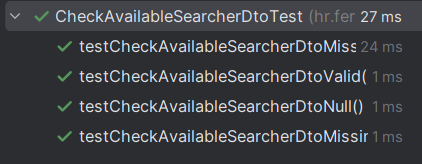
\includegraphics[scale=1]{slike/checkAvailableSearchersDtoTest.png} 
				\centering
				\caption{Rezultati ispitivanja}
				\label{fig:checkAvailableSearchersDtoTest}
			\end{figure}
			
			\subsection{Ispitivanje funkcije checkRequestDto:}
			Provjerava se funkcionalnost funkcije \textit{checkRequestDto} u \textit{ResearcherServiceJpa servisu} koja služi za provjeru ispravnosti podataka unutar \textit{RequestDto} objekta.
			
			\textbf{testCheckRequestDtoValid:}
			\begin{itemize}
				\item U funkciju se šalje objekt \textit{RequestDto} s ispravnim podacima.
				\item Očekuje se da neće doći do bacanja iznimke.
			\end{itemize}
			\begin{lstlisting}
				@Test
				public void testCheckRequestDtoValid() {
					RequestDto validRequestDto = new RequestDto();
					validRequestDto.setStationName("StationA");
					List<String> qualifications = Arrays.asList("QualificationA", "QualificationB");
					validRequestDto.setQualifications(qualifications);
					
					assertDoesNotThrow(() -> service.checkRequestDto(validRequestDto));
				}
			\end{lstlisting}
			
			\textbf{testCheckRequestDtoNull:}
			\begin{itemize}
				\item U funkciju se šalje objekt \textit{RequestDto} postavljen na \textit{null}.
				\item Očekuje se da će doći do bacanja iznimke.
			\end{itemize}
			\begin{lstlisting}
				@Test
				public void testCheckRequestDtoNull() {
					RequestDto nullRequestDto = null;
					
					IllegalArgumentException exception = assertThrows(IllegalArgumentException.class,
					() -> service.checkRequestDto(nullRequestDto));
					
					assertEquals("RequestDto is null", exception.getMessage());
				}
			\end{lstlisting}
			
			\textbf{testCheckRequestDtoMissingStationName:}
			\begin{itemize}
				\item U funkciju se šalje objekt \textit{RequestDto} s neispravnim podacima (nedostaje varijabla \textit{StationName}).
				\item Očekuje se da će doći do bacanja iznimke.
			\end{itemize}
			\begin{lstlisting}
				@Test
				public void testCheckRequestDtoMissingStationName() {
					RequestDto missingStationNameDto = new RequestDto();
					List<String> qualifications = Arrays.asList("QualificationA", "QualificationB");
					missingStationNameDto.setQualifications(qualifications);
					
					IllegalArgumentException exception = assertThrows(IllegalArgumentException.class,
					() -> service.checkRequestDto(missingStationNameDto));
					
					assertEquals("StationName is missing", exception.getMessage());
				}
			\end{lstlisting}
			
			\textbf{testCheckRequestDtoMissingQualifications:}
			\begin{itemize}
				\item U funkciju se šalje objekt \textit{RequestDto} s neispravnim podacima (nedostaje varijabla \textit{Qualifications}).
				\item Očekuje se da će doći do bacanja iznimke.
			\end{itemize}
			\begin{lstlisting}
				@Test
				public void testCheckRequestDtoMissingQualifications() {
					RequestDto missingQualificationsDto = new RequestDto();
					missingQualificationsDto.setStationName("StationA");
					
					IllegalArgumentException exception = assertThrows(IllegalArgumentException.class,
					() -> service.checkRequestDto(missingQualificationsDto));
					
					assertEquals("Qualifications is missing", exception.getMessage());
				}
			\end{lstlisting}
			
			\begin{figure}[H]
				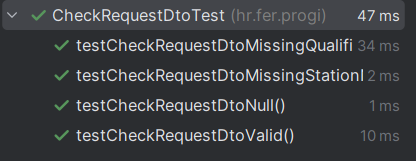
\includegraphics[scale=1]{slike/checkRequestDtoTest.png} 
				\centering
				\caption{Rezultati ispitivanja}
				\label{fig:checkRequestDtoTest}
			\end{figure}
			
			\subsection{Ispitivanje funkcije checkTaskDto:}
			Provjerava se funkcionalnost metode \textit{checkTaskDto} u \textit{taskServiceJpa servisu} koja služi za provjeru ispravnosti podataka unutar \textit{TaskDto} objekta.
			
			\textbf{testCheckTaskDtoValid:}
			\begin{itemize}
				\item U funkciju se šalje objekt \textit{TaskDto} s ispravnim podacima.
				\item Očekuje se da neće doći do bacanja iznimke.
			\end{itemize}
			\begin{lstlisting}
				@Test
				void testCheckTaskDtoValid() {
					TaskDto validTaskDto = new TaskDto(1L, 1L, new RouteWaypoints(), "TaskToDo", "TaskComment");
					assertDoesNotThrow(() -> taskServiceJpa.checkTaskDto(validTaskDto));
				}
			\end{lstlisting}
			
			\textbf{testCheckTaskDtoInvalidNull:}
			\begin{itemize}
				\item U funkciju se šalje objekt \textit{TaskDto} s neispravnim podacima (\textit{searcherId} postavljen na \textit{null}).
				\item Očekuje se da će doći do bacanja iznimke.
			\end{itemize}
			\begin{lstlisting}
				@Test
				public void testCheckActionDtoInvalidNull() {
					ActionDto invalidActionDto = new ActionDto(null, null, "ActionType", "LocationName");
					assertThrows(IllegalArgumentException.class, () -> researcherServiceJpa.checkActionDto(invalidActionDto));
				}
			\end{lstlisting}
			
			\textbf{testCheckTaskDtoInvalidEmpty:}
			\begin{itemize}
				\item U funkciju se šalje objekt \textit{TaskDto} s neispravnim podacima (\textit{taskToDo} postavljen na \textit{""}).
				\item Očekuje se da će doći do bacanja iznimke.
			\end{itemize}
			\begin{lstlisting}
				@Test
				void testCheckTaskDtoInvalidEmpty() {
					TaskDto invalidTaskDtoEmpty = new TaskDto(null, 1L, new RouteWaypoints(), "TaskComment", "");
					assertThrows(IllegalArgumentException.class, () -> taskServiceJpa.checkTaskDto(invalidTaskDtoEmpty));
				}
			\end{lstlisting}
			
			\textbf{testCheckTaskDtoInvalidWhitespace:}
			\begin{itemize}
				\item U funkciju se šalje objekt \textit{TaskDto} s neispravnim podacima (\textit{taskToDo} postavljen na \textit{"  TaskToDo"}).
				\item Očekuje se da će doći do bacanja iznimke.
			\end{itemize}
			\begin{lstlisting}
				@Test
				void testCheckTaskDtoInvalidWhitespace() {
					TaskDto invalidTaskDtoWhitespace = new TaskDto(null, 1L, new RouteWaypoints(), "TaskComment", "  TaskToDo");
					assertThrows(IllegalArgumentException.class, () -> taskServiceJpa.checkTaskDto(invalidTaskDtoWhitespace));
				}
			\end{lstlisting}
			
			\begin{figure}[H]
				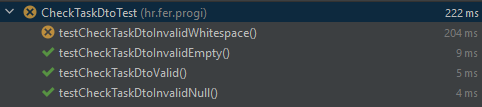
\includegraphics[scale=1]{slike/checkTaskDtoTest.png} 
				\centering
				\caption{Rezultati ispitivanja}
				\label{fig:promjene}
			\end{figure}
			
			\subsection{Ispitivanje funkcije emailRegexCheck:}
			Provjerava se funkcionalnost metode \textit{emailRegexCheck} u \textit{AuthenticationServiceJpa servisu} koja služi za provjeru ispravnog formata maila.
			
			\textbf{emailRegexCheckValidEmailReturnsTrue:}
			\begin{itemize}
				\item U funkciju se šalje mail ispravnog formata.
				\item Očekuje se da funkcija vraća true.
			\end{itemize}
			\begin{lstlisting}
			@Test
			void emailRegexCheck_ValidEmail_ReturnsTrue() {
				String validEmail = "test@example.com";
				boolean result = authenticationServiceJpa.emailRegexCheck(validEmail);
				assertTrue(result);
			}
			\end{lstlisting}
			
			\textbf{testEmailRegexCheckInvalidEmail:}
			\begin{itemize}
				\item U funkciju se šalje mail neispravnog formata.
				\item Očekuje se da funkcija vraća false.
			\end{itemize}
			\begin{lstlisting}
				@Test
				public void testEmailRegexCheckInvalidEmail() {
					String invalidEmail = "invalidemail";
					boolean isValid = authenticationServiceJpa.emailRegexCheck(invalidEmail);
					assertFalse(isValid);
				}
			\end{lstlisting}
			
			\textbf{testEmailRegexCheckInvalidEmailEdgeCase:}
			\begin{itemize}
				\item U funkciju se šalje mail neispravnog formata.
				\item Očekuje se da funkcija vraća false.
			\end{itemize}
			\begin{lstlisting}
				@Test
				public void testEmailRegexCheckInvalidEmail_EdgeCase() {
					String invalidEmail = "@.";
					boolean isValid = authenticationServiceJpa.emailRegexCheck(invalidEmail);
					assertFalse(isValid);
				}
			\end{lstlisting}
			\begin{figure}[H]
				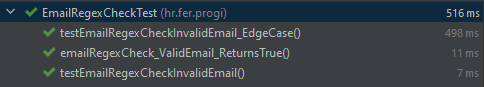
\includegraphics[scale=1]{slike/emailRegexTest.png} 
				\centering
				\caption{Rezultati ispitivanja}
				\label{fig:promjene}
			\end{figure}
			
			\subsection{Ispitivanje funkcije validateCoordinates:}
			Provjerava se funkcionalnost funkcije \textit{validateCoordinates} u \textit{CommentServiceJpa servisu} koja služi za provjeru ispravnosti koordinata koje prima ta klasa preko objekta \textit{MapCommentDto}.
			
			\textbf{testValidateCoordinatesValid:}
			\begin{itemize}
				\item U funkciju se šalje objekt \textit{MapCommentDto} s ispravnim podacima koordinata.
				\item Očekuje se da neće doći do bacanja iznimke.
			\end{itemize}
			\begin{lstlisting}
				@Test
				public void testValidateCoordinatesValid() {
					MapCommentDto validMapCommentDto = new MapCommentDto();
					List<Double> validCoordinates = Arrays.asList(1.0, 2.0, 3.0);
					validMapCommentDto.setCoordinates(validCoordinates);
					
					assertDoesNotThrow(() -> CommentServiceJpa.validateCoordinates(validMapCommentDto));
				}
			\end{lstlisting}
			
			\textbf{testValidateCoordinatesNullDto:}
			\begin{itemize}
				\item U funkciju se šalje objekt \textit{MapCommentDto} postavljen na \textit{null}.
				\item Očekuje se da će doći do bacanja iznimke.
			\end{itemize}
			\begin{lstlisting}
				@Test
				public void testValidateCoordinatesNullDto() {
					IllegalArgumentException exception = assertThrows(IllegalArgumentException.class,
					() -> CommentServiceJpa.validateCoordinates(null));
					
					assertEquals("Coordinates cannot be null", exception.getMessage());
				}
			\end{lstlisting}
			
			\textbf{testValidateCoordinatesNullCoordinate:}
			\begin{itemize}
				\item U funkciju se šalje objekt \textit{MapCommentDto} s jednom koordinatom postavljenom na \textit{null}.
				\item Očekuje se da će doći do bacanja iznimke.
			\end{itemize}
			\begin{lstlisting}
				@Test
				public void testValidateCoordinatesNullCoordinate() {
					MapCommentDto nullCoordinateDto = new MapCommentDto();
					List<Double> coordinatesWithNull = Arrays.asList(1.0, null, 3.0);
					nullCoordinateDto.setCoordinates(coordinatesWithNull);
					
					IllegalArgumentException exception = assertThrows(IllegalArgumentException.class,
					() -> CommentServiceJpa.validateCoordinates(nullCoordinateDto));
					
					assertEquals("Coordinate value cannot be null", exception.getMessage());
				}
			\end{lstlisting}
			
			\begin{figure}[H]
				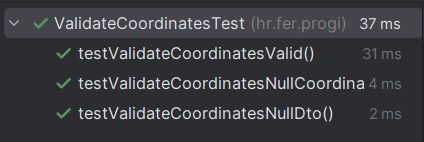
\includegraphics[scale=1]{slike/validateCoordinatesTest.png} 
				\centering
				\caption{Rezultati ispitivanja}
				\label{fig:validateCoordinatesTest}
			\end{figure}
			
			\subsection{Ispitivanje funkcije putRemoveFromAction:}
			Provjerava se funkcionalnost funkcije \textit{putRemoveFromAction} u \textit{SearcherInTheFieldJpa servisu} koja služi za micanje tragača s akcije.
			
			\textbf{testPutRemoveFromAction:}
			\begin{itemize}
				\item U funkciju se šalje \textit{appUserId} i vraća se mock objekt \textit{SearcherInTheField}.
				\item Očekuje se da neće doći do bacanja iznimke.
			\end{itemize}
			\begin{lstlisting}
				@Test
				public void testPutRemoveFromAction() {
					Long appUserId = 123L;
					
					SearcherInTheField searcherMock = mock(SearcherInTheField.class);
					
					when(searcherInTheFieldJpa.findByAppUserId(appUserId)).thenReturn(searcherMock);
					
					searcherInTheFieldJpa.putRemoveFromAction(appUserId);
					
					verify(searcherMock).setAction(null);
					verify(searcherMock).setCurrentPosition(null);
					
					verify(pastDataServiceJpa).searcherPositionSave(searcherMock);
					
					verify(searcherInTheFieldRepository).save(searcherMock);
				}
			\end{lstlisting}
			
			\textbf{testPutRemoveFromAction\_AppUserNotFound:}
			\begin{itemize}
				\item U funkciju se šalje \textit{appUserId} i vraća se objekt \textit{SearcherInTheField} postavljen na \textit{null}.
				\item Očekuje se da će doći do bacanja iznimke.
			\end{itemize}
			\begin{lstlisting}
				@Test
				public void testPutRemoveFromAction_AppUserNotFound() {
					Long appUserId = 123L;
					
					when(searcherInTheFieldJpa.findByAppUserId(appUserId)).thenReturn(null);
					
					IllegalArgumentException exception = assertThrows(IllegalArgumentException.class,
					() -> searcherInTheFieldJpa.putRemoveFromAction(appUserId));
					
					assertEquals("SearcherInTheField is null", exception.getMessage());
					
					verifyNoMoreInteractions(searcherInTheFieldRepository, pastDataServiceJpa);
				}
			\end{lstlisting}
			
			\textbf{testPutRemoveFromAction\_SaveFailure:}
			\begin{itemize}
				\item U funkciju se šalje \textit{appUserId} i vraća se objekt \textit{SearcherInTheField} postavljen na \textit{null}. Provjerava se ponašanje funkcije kada spremanje u repozitorij nije uspješno tj. vraća \textit{null}.
				\item Očekuje se da neće doći do bacanja iznimke.
			\end{itemize}
			\begin{lstlisting}
				@Test
				public void testPutRemoveFromAction_SaveFailure() {
					Long appUserId = 123L;
					
					SearcherInTheField searcherMock = mock(SearcherInTheField.class);
					
					when(searcherInTheFieldJpa.findByAppUserId(appUserId)).thenReturn(searcherMock);
					when(searcherInTheFieldRepository.save(searcherMock)).thenReturn(null);
					
					searcherInTheFieldJpa.putRemoveFromAction(appUserId);
					
					verify(pastDataServiceJpa).searcherPositionSave(searcherMock);
					
					verify(searcherInTheFieldRepository).save(searcherMock);
				}
			\end{lstlisting}
			
			\begin{figure}[H]
				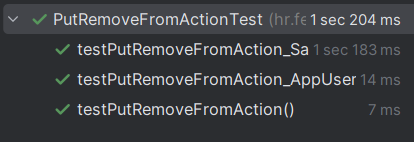
\includegraphics[scale=1]{slike/putRemoveFromActionTest.png} 
				\centering
				\caption{Rezultati ispitivanja}
				\label{fig:putRemoveFromActionTest}
			\end{figure}
			
			
			\section{Ispitivanje sustava}
			
			
			Sustav smo detaljno testirali primjenom Selenium WebDriver dodatka unutar JUnit testova. Proveli smo dva ključna ispitivanja kako bismo osigurali funkcionalnost sustava: jedno je bilo usmjereno na proces prijave korisnika, dok je drugo obuhvatilo postupak registracije.
			
			\subsection{Ispitivanje Prijave Korisnika:}
			\textbf{testLoginValidCreds:}
			\begin{itemize}
				\item Unose se ispravne korisničke akreditacije (valjana e-mail adresa i lozinka).
				\item Provjerava se preusmjeravanje nakon prijave.
				\item Očekuje se da je korisnik uspješno preusmjeren na "dashboard".
			\end{itemize}
			\begin{lstlisting}
			@Test
			public void testLogin_ValidCreds(){
				ChromeOptions options = new ChromeOptions();
				options.addArguments("--remote-allow-origins=*");
				WebDriver driver = new ChromeDriver(options);
				driver.manage().timeouts().implicitlyWait(10, TimeUnit.SECONDS);
				driver.get("https://wildtrack-fe.onrender.com/login");
				
				WebElement element = driver.findElement(By.name("email"));
				element.sendKeys("admin@wildtrack.com");
				element = driver.findElement(By.name("password"));
				element.sendKeys("admin123");
				driver.findElement(By.cssSelector(".login-button")).click();
				
				try {
					Thread.sleep(5000);
				} catch (InterruptedException e) {
					e.printStackTrace();
				}
				String redirURL = driver.getCurrentUrl();
				boolean compRes = redirURL.contains("dashboard");
				
				assertEquals(compRes, true);
				
				driver.quit();
			}
			\end{lstlisting}
			
			\textbf{testLoginInValidCreds:}
			\begin{itemize}
				\item Unose se nevaljane korisničke akreditacije (neispravna e-mail adresa i lozinka).
				\item Provjerava se preusmjeravanje nakon pokušaja prijave.
				\item Očekuje se da korisnik nije preusmjeren na "dashboard".
			\end{itemize}
			\begin{lstlisting}
				@Test
				public void testLogin_InvalidCreds(){
					ChromeOptions options = new ChromeOptions();
					options.addArguments("--remote-allow-origins=*");
					WebDriver driver = new ChromeDriver(options);
					driver.manage().timeouts().implicitlyWait(10, TimeUnit.SECONDS);
					driver.get("https://wildtrack-fe.onrender.com/login");
					
					WebElement element = driver.findElement(By.name("email"));
					element.sendKeys("invalid");
					element = driver.findElement(By.name("password"));
					element.sendKeys("invalid");
					driver.findElement(By.cssSelector(".login-button")).click();
					
					String redirURL = driver.getCurrentUrl();
					boolean compRes = redirURL.contains("dashboard");
					
					assertEquals(compRes, false);
					
					driver.quit();
				}
			\end{lstlisting}
			
			\textbf{testLoginEmptyEmail:}
			\begin{itemize}
				\item Ostavlja se polje za e-mail prazno.
				\item Postavlja se lozinka na neku vrijednost.
				\item Provjerava se preusmjeravanje nakon pokušaja prijave.
				\item Očekuje se da korisnik nije preusmjeren na "dashboard".
			\end{itemize}
			\begin{lstlisting}
				@Test
				public void testLogin_emptyEmail() {
					ChromeOptions options = new ChromeOptions();
					options.addArguments("--remote-allow-origins=*");
					WebDriver driver = new ChromeDriver(options);
					driver.manage().timeouts().implicitlyWait(10, TimeUnit.SECONDS);
					driver.get("https://wildtrack-fe.onrender.com/login");

					WebElement emailElement = driver.findElement(By.name("email"));
					emailElement.sendKeys("");
					
					WebElement passwordElement = driver.findElement(By.name("password"));
					passwordElement.sendKeys("somePassword");
					
					driver.findElement(By.cssSelector(".login-button")).click();
					
					String redirURL = driver.getCurrentUrl();
					boolean compRes = redirURL.contains("dashboard");
					
					assertEquals(compRes, false);
					
					driver.quit();
				}
			\end{lstlisting}
			
			\begin{figure}[H]
				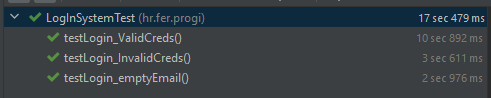
\includegraphics[scale=1]{slike/loginTests.png} 
				\centering
				\caption{Rezultati ispitivanja}
				\label{fig:promjene}
			\end{figure}
			
			Drugo ispitivanje bilo je usmjereno na proces registracije novog korisnika. Kroz Selenium WebDriver testove, simulirali smo korisničko sučelje kako bismo provjerili ispravnost postupka registracije. Cilj je bio osigurati da sustav adekvatno obrađuje unos novih korisničkih podataka te da novi korisnik bude uspješno registriran u sustavu.
			
			\textit{Ključne Točke Ispitivanja:}
			\begin{itemize}
				\item Popunjavanje obrasca za registraciju s valjanim podacima.
				\item Klik na gumb za registraciju.
				\item Provjera uspješne registracije i ispravnosti prelaska na stranicu nakon registracije.
			\end{itemize}
			
			\subsection{Ispitivanje Registracije:}
			\textbf{testRegistrationInvalidCreds:}
			\begin{itemize}
				\item Unosi se email u neispravnom formatu.
				\item Provjerava se ispisan tekst na stranici.
				\item Očekuje se je da je na stranici ispisan tekst \textit{email not valid}.
			\end{itemize}
			\begin{lstlisting}
				@Test
				public void testRegistration_InvalidCreds(){
					ChromeOptions options = new ChromeOptions();
					options.addArguments("--remote-allow-origins=*");
					WebDriver driver = new ChromeDriver(options);
					driver.manage().timeouts().implicitlyWait(10, TimeUnit.SECONDS);
					driver.get("https://wildtrack-fe.onrender.com/register");
					
					WebElement firstNameInput = driver.findElement(By.id("register-firstName"));
					firstNameInput.sendKeys("test");
					
					WebElement lastNameInput = driver.findElement(By.id("register-lastName"));
					lastNameInput.sendKeys("test");
					
					WebElement usernameInput = driver.findElement(By.id("register-username"));
					usernameInput.sendKeys("test");
					
					WebElement emailInput = driver.findElement(By.id("register-email"));
					emailInput.sendKeys("test");
					
					WebElement passwordInput = driver.findElement(By.id("register-password"));
					passwordInput.sendKeys("test");
					
					WebElement tragacRadioButton = driver.findElement(By.id("register-searcher"));
					tragacRadioButton.click();
					
					WebElement fileInput = driver.findElement(By.id("photo-upload"));
					fileInput.sendKeys("D:\\FER-predmeti\\zoolanders\\zoolanders\\be\\src
					\\test\\resources\\profile.jpg");
					
					WebElement registerButton = driver.findElement(By.cssSelector(".register-button"));
					registerButton.click();
					
					try {
						Thread.sleep(10000);
					} catch (InterruptedException e) {
						e.printStackTrace();
					}
					WebElement errorElement = driver.findElement(By.className("register-error"));
					String actualErrorText = errorElement.getText();
					String expectedErrorText = "email not valid";
					
					assertEquals(expectedErrorText, actualErrorText);
					
					driver.quit();
				}
			\end{lstlisting}
			
			\textbf{testRegistrationEmailAllReadyTaken:}
			\begin{itemize}
				\item Unose se korisnički podaci u ispravnom formatu.
				\item Provjerava se ispisan tekst na stranici.
				\item Očekuje se je da je na stranici ispisan tekst \textit{email already taken}.
			\end{itemize}
			\begin{lstlisting}
				@Test
				public void testRegistration_InvalidCreds(){
					ChromeOptions options = new ChromeOptions();
					options.addArguments("--remote-allow-origins=*");
					WebDriver driver = new ChromeDriver(options);
					driver.manage().timeouts().implicitlyWait(10, TimeUnit.SECONDS);
					driver.get("https://wildtrack-fe.onrender.com/register");
					
					WebElement firstNameInput = driver.findElement(By.id("register-firstName"));
					firstNameInput.sendKeys("test");
					
					WebElement lastNameInput = driver.findElement(By.id("register-lastName"));
					lastNameInput.sendKeys("test");
					
					WebElement usernameInput = driver.findElement(By.id("register-username"));
					usernameInput.sendKeys("test");
					
					WebElement emailInput = driver.findElement(By.id("register-email"));
					emailInput.sendKeys("test");
					
					WebElement passwordInput = driver.findElement(By.id("register-password"));
					passwordInput.sendKeys("test");
					
					WebElement tragacRadioButton = driver.findElement(By.id("register-searcher"));
					tragacRadioButton.click();
					
					WebElement fileInput = driver.findElement(By.id("photo-upload"));
					fileInput.sendKeys("D:\\FER-predmeti\\zoolanders\\zoolanders\\be\\src
					\\test\\resources\\profile.jpg");
					
					WebElement registerButton = driver.findElement(By.cssSelector(".register-button"));
					registerButton.click();
					
					try {
						Thread.sleep(10000);
					} catch (InterruptedException e) {
						e.printStackTrace();
					}
					WebElement errorElement = driver.findElement(By.className("register-error"));
					String actualErrorText = errorElement.getText();
					String expectedErrorText = "email not valid";
					
					assertEquals(expectedErrorText, actualErrorText);
					
					driver.quit();
				}
			\end{lstlisting}
			
			\textbf{testRegistrationValidCreds:}
			\begin{itemize}
				\item Unose se korisnički podaci u ispravnom formatu.
				\item Provjerava se ispisan tekst na stranici.
				\item Očekuje se je da je na stranici ispisan tekst \textit{Registracija uspješna!}.
			\end{itemize}
			\begin{lstlisting}
				@Test
				public void testRegistration_ValidCreds(){
					ChromeOptions options = new ChromeOptions();
					options.addArguments("--remote-allow-origins=*");
					WebDriver driver = new ChromeDriver(options);
					driver.manage().timeouts().implicitlyWait(10, TimeUnit.SECONDS);
					driver.get("https://wildtrack-fe.onrender.com/register");
					
					WebElement firstNameInput = driver.findElement(By.id("register-firstName"));
					firstNameInput.sendKeys("test");
					
					WebElement lastNameInput = driver.findElement(By.id("register-lastName"));
					lastNameInput.sendKeys("test");
					
					WebElement usernameInput = driver.findElement(By.id("register-username"));
					usernameInput.sendKeys("test");
					
					WebElement emailInput = driver.findElement(By.id("register-email"));
					emailInput.sendKeys("test1@test.com");
					
					WebElement passwordInput = driver.findElement(By.id("register-password"));
					passwordInput.sendKeys("test");
					
					WebElement tragacRadioButton = driver.findElement(By.id("register-searcher"));
					tragacRadioButton.click();
					
					WebElement fileInput = driver.findElement(By.id("photo-upload"));
					fileInput.sendKeys("D:\\FER-predmeti\\zoolanders\\zoolanders\\be\\src
					\\test\\resources\\profile.jpg");
					
					WebElement registerButton = driver.findElement(By.cssSelector(".register-button"));
					registerButton.click();
					
					try {
						Thread.sleep(10000);
					} catch (InterruptedException e) {
						e.printStackTrace();
					}
					WebElement errorElement = driver.findElement(By.className("register-success"));
					String actualText = errorElement.getText();
 					String expectedText = "Registracija uspjesna!";
					
					assertEquals(expectedText, actualText);
					
					driver.quit();
				}
			\end{lstlisting}
			
			\begin{figure}[H]
				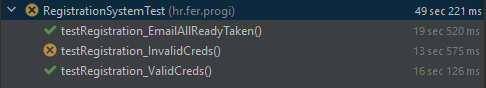
\includegraphics[scale=1]{slike/registrationTests.png} 
				\centering
				\caption{Rezultati ispitivanja}
				\label{fig:promjene}
			\end{figure}
			
			\eject 
		
		
		\section{Dijagram razmještaja}
			
			\textbf{\textit{dio 2. revizije}}
			
			 \textit{Potrebno je umetnuti \textbf{specifikacijski} dijagram razmještaja i opisati ga. Moguće je umjesto specifikacijskog dijagrama razmještaja umetnuti dijagram razmještaja instanci, pod uvjetom da taj dijagram bolje opisuje neki važniji dio sustava.}
			
			\eject 
		
		\section{Upute za puštanje u pogon}
		
			U ovom poglavlju prikazat ćemo kako se provodi pokretanje aplikacije na lokalnom računalu.
			
			\textbf{Instalacija a posluzitelja baze podataka}
			Potrebno je preuzeti PostgreSQL bazu podataka (za operacijski sustav Windows). Instalacij se može provesti pomoću ovoga linka https://www.postgresql.org/download/. Prilikom instalacije zapamtite koji ste vrata (engl. port) stavili za pristup bazi podataka pošto će nam trebati kasnije(predložena su vrata 5432). Nakon provedene instalacije na računalu će se nalaziti PostgreSQL baza podataka.
			
			\textbf{Konfiguracija baze podataka}
			Za daljnju konfiguraciju i baze podataka i ostatak projekta koristiti ćemo Inetllij IDE. Prije svega s github repozitorija https://github.com/filip-ljubotina/zoolanders.git preuzet ćemo projekt, te u Intellij-u u gornjem lijevo kutu odabiremo File -> Open... te se pozicijoniramo u be direktorij projekta. Sljedeće kao što je prikazano na slici odabire izvor podataka (engl. Data Source).
			
			\begin{figure}[H]
				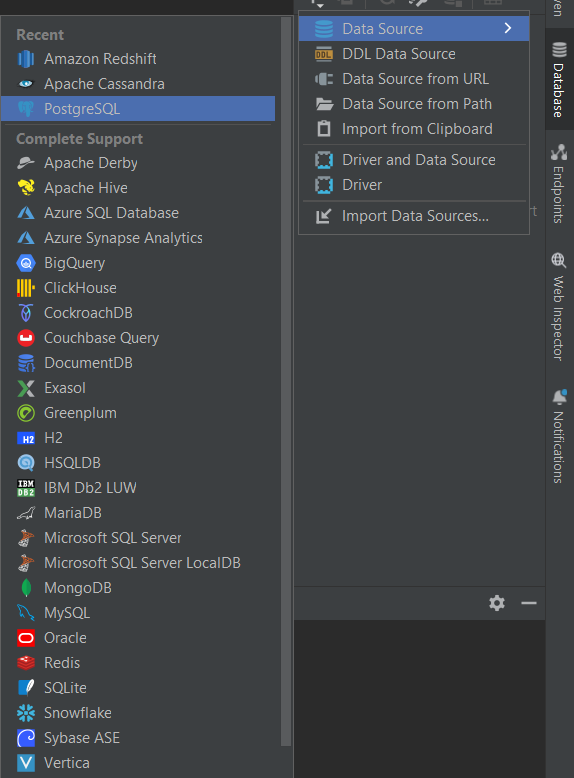
\includegraphics[scale=0.3]{slike/postgreSql.png} 
				\centering
				\caption{Odabir izvora podataka}
				\label{fig:promjene}
			\end{figure}
			Nakon odabira PostgreSQL-a kao izvor podataka potrebno je unjeti podatke o bazi podataka gdje za user stavljamo postrges, a port i password su isti kao što smo ih postavili tokom instalacije.
			
			\textbf{Punjenje baze podataka}
			Nakon konfiguracije baze podataka potrebno je napuniti istu. To također radimo unutar Intellij-a tako što desnim klikom na postregs bazu odabiremo Run Sql Script kao što je prikazano na slici. Zatim odabiremo skriptu koja se nalazi u direktoriju projekta, te će se nakon pokretanja baza napuniti s pocetnim podacima.
			
			\begin{figure}[H]
				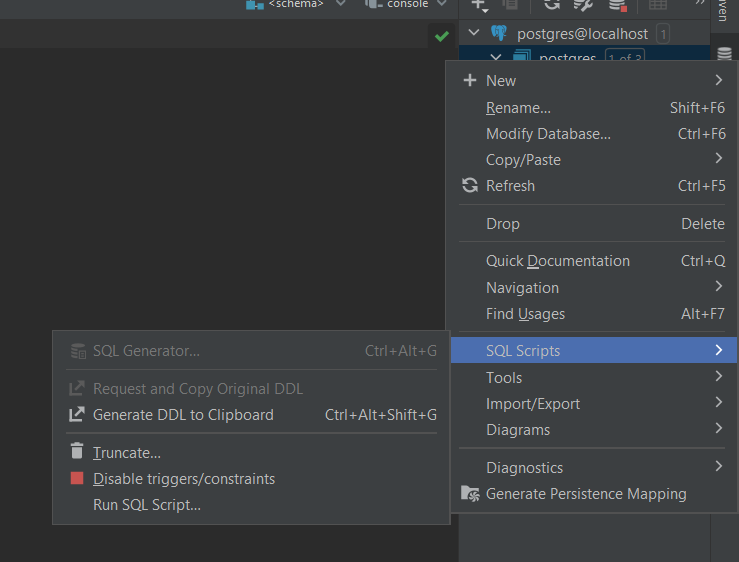
\includegraphics[scale=0.3]{slike/runSqlScript.png} 
				\centering
				\caption{Pokretanje SQL skripte}
				\label{fig:promjene}
			\end{figure}
			
			\textbf{Konfiguracija frontend-a i backend-a}
			Nakon postavljene baze podataka sljedeće konfiguriramo backend. Potrebno je otici u application.yaml file u resources paketu, te postaviti password username i url od datasource-a da butu isti kao što su bili postavljeni pri konfiguraciji datasource-a. Za konfiguraciju frontend-a potrebno je otviri u fe direktorij te u services -> ApiService postaviti baseURL na "http://localhost:8080". Zatim u command prompt-u potrebno j pozicionirati se u fe direktorij te pokrenuti naredbu nmp install.
			
			\textbf{Pokretanje aplikacije}
			Za pokretanje backenda u Intellij-eju je potrebno pokrenuti WildtrackApplication, a za frontend u terminalu je potrebnu pokrenuti naredbu npm start.
			
			\eject 